\documentclass[french, 12pt]{article}
\usepackage[a4paper, top=2cm, bottom=2cm, left=2cm, right=2cm]{geometry}

\usepackage{fancyvrb}

\usepackage[T1]{fontenc}
\usepackage[french]{babel}

\usepackage{graphicx}
\usepackage{circuitikz}

\begin{document}

\section*{Fonctionnement du main}

Le fichier main.py s'occupe de définir le pc, les registres, les flags, et la ROM. À chaque cycle il recupère toutes les anciennes valeurs grâce à des REG, fait appels aux différents modules et selectionne la valeur souhaitée parmi les résultats renvoyés.

Les différents modules appelés sont :
\begin{itemize}
    \item l'alu
    \item les décalages de bits
    \item les opérations sur la RAM
    \item les saut dans le programme
\end{itemize}

Le circuit logique simplifié correspondant au main est donc :

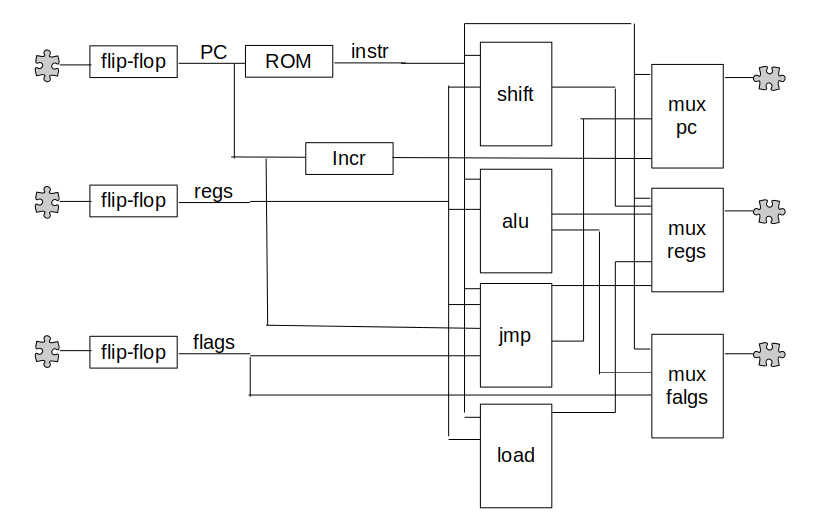
\includegraphics[width=17cm]{circuit_main.png}


\end{document}
